\documentclass{standalone}
\usepackage{pgfplots}

\begin{document}
	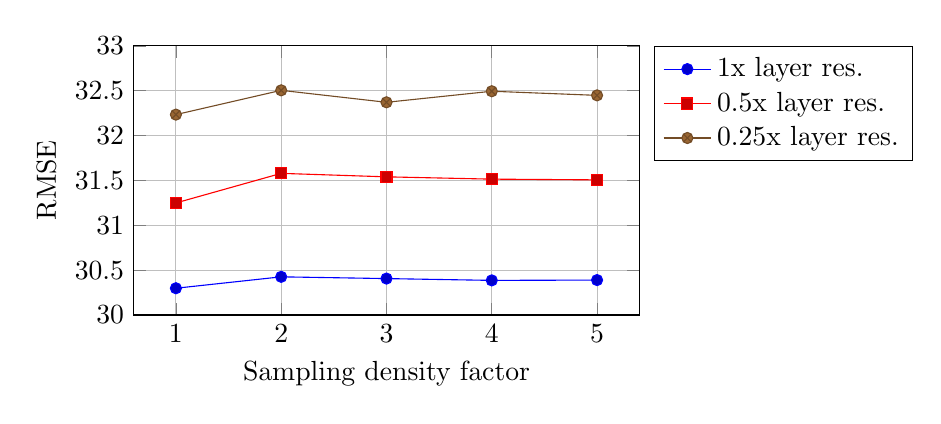
\begin{tikzpicture}
		
		\begin{axis}[	xtick = {1, 2, 3, 4, 5},
						ymin = 30, 
						ymax = 33,
						ytick = {30.0, 30.5, 31.0, 31.5, 32.0, 32.5, 33.0},
						ylabel = {RMSE},
						xlabel = {Sampling density factor},
						ylabel near ticks,
						grid = major,
						axis on top = false,
						width = 8 cm, 
						height = 5cm, 
						legend cell align = left,
						legend pos = outer north east]
		
			\addplot coordinates { 
				(1, 	30.2980)
				(2, 	30.4251)
				(3, 	30.4056)
				(4, 	30.3855)
				(5, 	30.3890)
			};
			\addlegendentry{1x layer res.};

			\addplot coordinates {
				(1, 	31.2485)
				(2, 	31.5784)
				(3, 	31.5396)
				(4, 	31.5140)
				(5, 	31.5059)
			};
			\addlegendentry{0.5x layer res.};
			
			\addplot coordinates {
				(1, 	32.2331) 
				(2, 	32.5038)
				(3, 	32.3703)
				(4, 	32.4936)
				(5, 	32.4477)
			};
			\addlegendentry{0.25x layer res.};			
			 
		\end{axis}
		
	\end{tikzpicture}
\end{document}